\documentclass[11pt,a4paper]{article}
\usepackage[utf8]{inputenc}
\usepackage[T1]{fontenc}
\usepackage{geometry}
\usepackage{fancyhdr}
\usepackage{graphicx}
\usepackage{xcolor}
\usepackage{listings}
\usepackage{hyperref}
\usepackage{tikz}
\usepackage{booktabs}
\usepackage{longtable}
\usepackage{enumitem}

\geometry{margin=2.5cm}

\definecolor{codegreen}{rgb}{0,0.6,0}
\definecolor{codegray}{rgb}{0.5,0.5,0.5}
\definecolor{codepurple}{rgb}{0.58,0,0.82}
\definecolor{backcolour}{rgb}{0.95,0.95,0.92}
\definecolor{alertred}{rgb}{0.8,0.1,0.1}

\lstdefinestyle{mystyle}{
    backgroundcolor=\color{backcolour},   
    commentstyle=\color{codegreen},
    keywordstyle=\color{magenta},
    numberstyle=\tiny\color{codegray},
    stringstyle=\color{codepurple},
    basicstyle=\ttfamily\footnotesize,
    breakatwhitespace=false,         
    breaklines=true,                 
    captionpos=b,                    
    keepspaces=true,                 
    numbers=left,                    
    numbersep=5pt,                  
    showspaces=false,                
    showstringspaces=false,
    showtabs=false,                  
    tabsize=2
}

\lstset{style=mystyle}

\pagestyle{fancy}
\fancyhf{}
\rhead{DVD Security Guide}
\lhead{Defensive Measures}
\rfoot{Page \thepage}

\begin{document}

\title{\textbf{Damn Vulnerable Drone} \\ Security Analysis \& Defensive Measures \\ \large{Comprehensive Defense Guide}}
\author{Cybersecurity Research Team}
\date{\today}

\maketitle

\tableofcontents
\newpage

\section{Executive Summary}

Dieses Dokument analysiert die Sicherheitslücken im Damn Vulnerable Drone (DVD) System und bietet umfassende Verteidigungsstrategien für reale Implementierungen. Während das DVD-System bewusst Schwachstellen für Bildungszwecke enthält, zeigen die hier beschriebenen Gegenmaßnahmen, wie entsprechende Produktionssysteme abgesichert werden können.

\subsection{Kritische Erkenntnisse}

\begin{itemize}[leftmargin=*]
    \item Supply Chain Angriffe stellen eine erhebliche Bedrohung für kritische Infrastrukturen dar
    \item Schwache Zugriffskontrollen können zu vollständiger Systemkompromittierung führen
    \item Ungesicherte Build-Pipelines ermöglichen persistente Angriffe
    \item Fehlende Monitoring-Mechanismen verzögern die Erkennung von Kompromittierungen
\end{itemize}

\section{Bedrohungsmodell}

\subsection{Angreifer-Profile}

\begin{longtable}{|l|p{4cm}|p{3cm}|p{4cm}|}
\caption{Potenzielle Angreifer und ihre Fähigkeiten} \\
\hline
\textbf{Angreifer-Typ} & \textbf{Motivation} & \textbf{Fähigkeiten} & \textbf{Ressourcen} \\
\hline
\endfirsthead
\hline
\textbf{Angreifer-Typ} & \textbf{Motivation} & \textbf{Fähigkeiten} & \textbf{Ressourcen} \\
\hline
\endhead
\hline
\endfoot
\hline
\endlastfoot

Script Kiddie & Neugierde, Reputation & Basic Tools, Tutorials & Begrenzt \\
\hline
Insider Threat & Rache, finanzieller Gewinn & Systemzugang, Domain-Wissen & Mittel \\
\hline
Cyberkriminelle & Finanzieller Gewinn & Fortgeschrittene Tools & Hoch \\
\hline
Nation State & Spionage, Sabotage & APT-Tools, Zero-Days & Sehr hoch \\
\hline
Terrorist & Disruption, Schaden & Variable & Variable \\
\hline
\end{longtable}

\subsection{Attack Vectors}

\begin{figure}[h]
\centering
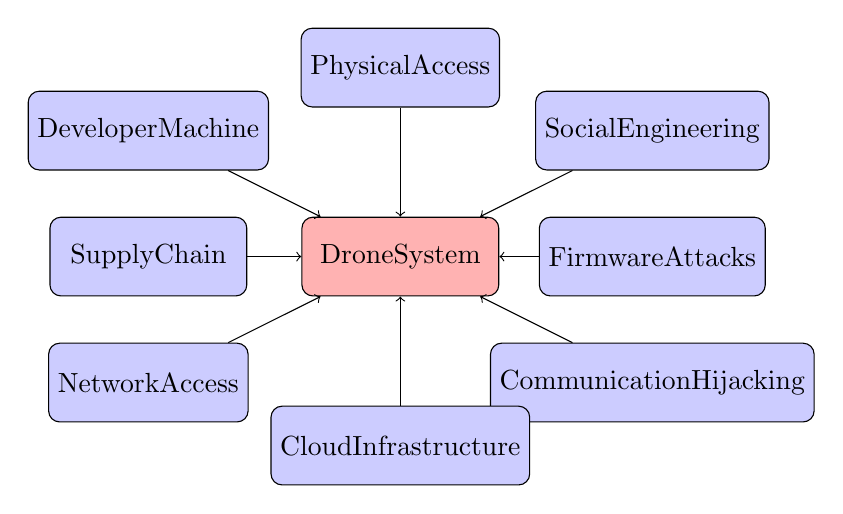
\begin{tikzpicture}[scale=0.8, every node/.style={draw, rectangle, rounded corners, text centered, minimum width=2.5cm, minimum height=1cm}]
    
    % Central target
    \node[fill=red!30] (target) at (0,0) {Drone\\System};
    
    % Attack vectors
    \node[fill=blue!20] (dev) at (-4,2) {Developer\\Machine};
    \node[fill=blue!20] (supply) at (-4,0) {Supply\\Chain};
    \node[fill=blue!20] (network) at (-4,-2) {Network\\Access};
    \node[fill=blue!20] (physical) at (0,3) {Physical\\Access};
    \node[fill=blue!20] (social) at (4,2) {Social\\Engineering};
    \node[fill=blue!20] (firmware) at (4,0) {Firmware\\Attacks};
    \node[fill=blue!20] (comm) at (4,-2) {Communication\\Hijacking};
    \node[fill=blue!20] (cloud) at (0,-3) {Cloud\\Infrastructure};
    
    % Arrows
    \draw[->] (dev) -- (target);
    \draw[->] (supply) -- (target);
    \draw[->] (network) -- (target);
    \draw[->] (physical) -- (target);
    \draw[->] (social) -- (target);
    \draw[->] (firmware) -- (target);
    \draw[->] (comm) -- (target);
    \draw[->] (cloud) -- (target);
    
\end{tikzpicture}
\caption{Potenzielle Angriffsvektoren auf Drohnensysteme}
\end{figure}

\section{Schwachstellenanalyse}

\subsection{Identifizierte Sicherheitslücken}

\begin{longtable}{|l|l|p{3cm}|l|l|}
\caption{Detaillierte Schwachstellenanalyse} \\
\hline
\textbf{ID} & \textbf{Komponente} & \textbf{Schwachstelle} & \textbf{CVSS} & \textbf{Priorität} \\
\hline
\endfirsthead
\hline
\textbf{ID} & \textbf{Komponente} & \textbf{Schwachstelle} & \textbf{CVSS} & \textbf{Priorität} \\
\hline
\endhead
\hline
\endfoot
\hline
\endlastfoot

DVD-001 & Developer Machine & Sudo NOPASSWD crontab & 8.8 & Critical \\
\hline
DVD-002 & Shared Builds & Unsecured file permissions & 7.5 & High \\
\hline
DVD-003 & Build Pipeline & No integrity verification & 8.1 & Critical \\
\hline
DVD-004 & Network & Unencrypted MAVLink & 6.5 & Medium \\
\hline
DVD-005 & Authentication & Weak passwords & 7.8 & High \\
\hline
DVD-006 & Logging & Insufficient audit trails & 5.4 & Medium \\
\hline
DVD-007 & Container & Privileged capabilities & 7.2 & High \\
\hline
\end{longtable}

\subsection{Angriffsketten-Analyse}

\subsubsection{Primary Attack Chain: Supply Chain Compromise}

\begin{enumerate}[leftmargin=*]
    \item \textbf{Initial Access:} Schwache Anmeldedaten (developer:dev123)
    \item \textbf{Privilege Escalation:} Ausnutzung von sudo crontab NOPASSWD
    \item \textbf{Persistence:} Installation von malicious cron jobs
    \item \textbf{Collection:} Discovery von Build-Artefakten
    \item \textbf{Impact:} Manipulation kritischer Drohnen-Software
\end{enumerate}

\subsubsection{Secondary Attack Chain: Network-based}

\begin{enumerate}[leftmargin=*]
    \item \textbf{Reconnaissance:} Netzwerk-Scanning und Service-Enumeration
    \item \textbf{Initial Access:} Exploitation von exponierten Services
    \item \textbf{Lateral Movement:} Container-to-Container-Kommunikation
    \item \textbf{Command \& Control:} Reverse Shell über MAVLink
    \item \textbf{Impact:} Direkte Drohnen-Kontrolle
\end{enumerate}

\section{Defensive Strategien}

\subsection{Defense in Depth}

Das Konzept der mehrstufigen Verteidigung ist essentiell für die Absicherung von Drohnensystemen:

\begin{figure}[h]
\centering
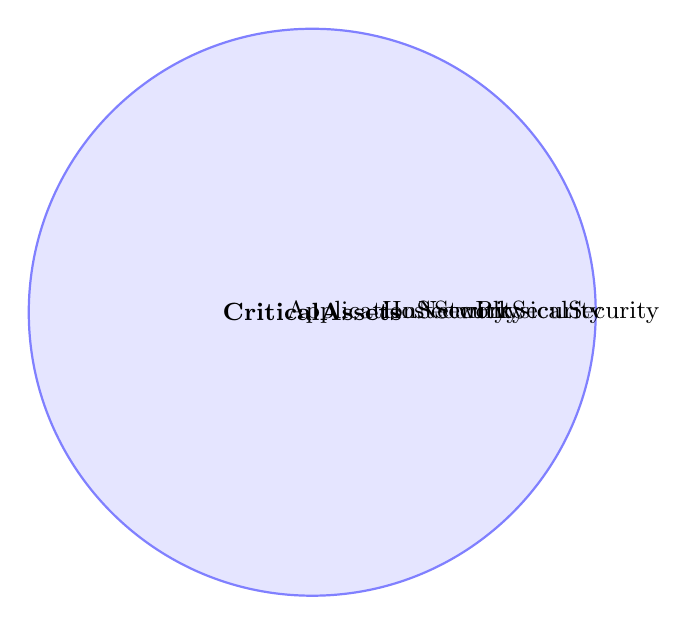
\begin{tikzpicture}[scale=0.9]
    % Concentric circles for defense layers
    \draw[thick, red!30, fill=red!10] (0,0) circle (0.8cm);
    \draw[thick, orange!50, fill=orange!10] (0,0) circle (1.6cm);
    \draw[thick, yellow!70, fill=yellow!10] (0,0) circle (2.4cm);
    \draw[thick, green!50, fill=green!10] (0,0) circle (3.2cm);
    \draw[thick, blue!50, fill=blue!10] (0,0) circle (4.0cm);
    
    % Labels
    \node at (0,0) {\small\textbf{Critical\\Assets}};
    \node at (1.2,0) {\small Application\\Security};
    \node at (2.0,0) {\small Host\\Security};
    \node at (2.8,0) {\small Network\\Security};
    \node at (3.6,0) {\small Physical\\Security};
    
\end{tikzpicture}
\caption{Defense in Depth Modell für Drohnensysteme}
\end{figure}

\subsection{Prioritäre Sicherheitsmaßnahmen}

\subsubsection{1. Zugriffskontrolle und Authentifizierung}

\begin{lstlisting}[language=bash, caption=Sichere Benutzer-Konfiguration]
# Entfernung von sudo NOPASSWD
sed -i '/NOPASSWD/d' /etc/sudoers

# Implementierung starker Passwort-Richtlinien
apt-get install libpam-pwquality
echo "password requisite pam_pwquality.so retry=3 minlen=12 \
  difok=3 ucredit=-1 lcredit=-1 dcredit=-1 ocredit=-1" \
  >> /etc/pam.d/common-password

# Multi-Faktor-Authentifizierung
apt-get install libpam-google-authenticator
echo "auth required pam_google_authenticator.so" \
  >> /etc/pam.d/sshd
\end{lstlisting}

\subsubsection{2. Build-Pipeline-Sicherheit}

\begin{lstlisting}[language=yaml, caption=Sichere CI/CD-Pipeline]
# .github/workflows/secure-build.yml
name: Secure Build Pipeline

on: [push, pull_request]

jobs:
  security-scan:
    runs-on: ubuntu-latest
    steps:
      - uses: actions/checkout@v3
      
      # Static Code Analysis
      - name: Run CodeQL Analysis
        uses: github/codeql-action/analyze@v2
        
      # Dependency Scanning
      - name: Run Snyk Security Scan
        uses: snyk/actions/docker@master
        env:
          SNYK_TOKEN: ${{ secrets.SNYK_TOKEN }}
          
      # Container Security
      - name: Run Trivy Scanner
        uses: aquasecurity/trivy-action@master
        with:
          image-ref: 'dvd-developer-machine:latest'
          format: 'sarif'
          
      # Code Signing
      - name: Sign Artifacts
        uses: sigstore/cosign-installer@v2
        with:
          cosign-release: 'v1.13.1'
\end{lstlisting}

\subsubsection{3. Container-Härtung}

\begin{lstlisting}[language=dockerfile, caption=Gehärteter Container]
FROM ubuntu:22.04

# Non-root User erstellen
RUN groupadd -r dvduser && useradd -r -g dvduser dvduser

# Sichere Basis-Konfiguration
RUN apt-get update && apt-get install -y --no-install-recommends \
    ca-certificates \
    && rm -rf /var/lib/apt/lists/* \
    && apt-get purge -y --auto-remove

# Security-optimierte Einstellungen
USER dvduser
WORKDIR /app

# Read-only Root Filesystem
VOLUME ["/tmp", "/var/log"]

# Health Check
HEALTHCHECK --interval=30s --timeout=3s --start-period=5s \
  --retries=3 CMD curl -f http://localhost/ || exit 1

# Security Labels
LABEL security.scan-policy="enabled"
LABEL security.vulnerability-scan="required"
\end{lstlisting}

\subsubsection{4. Netzwerk-Segmentierung}

\begin{lstlisting}[language=yaml, caption=Mikro-Segmentierung mit Docker Networks]
# docker-compose-secure.yml
version: '3.8'

services:
  developer-machine:
    networks:
      - dev-network
    
  ground-control:
    networks:
      - control-network
      - drone-network
    
  drone-simulation:
    networks:
      - drone-network

networks:
  dev-network:
    driver: bridge
    internal: true
    ipam:
      config:
        - subnet: 172.30.1.0/24
  
  control-network:
    driver: bridge
    ipam:
      config:
        - subnet: 172.30.2.0/24
        
  drone-network:
    driver: bridge
    ipam:
      config:
        - subnet: 172.30.3.0/24
\end{lstlisting}

\section{Monitoring und Detection}

\subsection{SIEM-Integration}

\begin{lstlisting}[language=bash, caption=ELK Stack für Security Monitoring]
# Elasticsearch, Logstash, Kibana Setup
docker run -d --name elasticsearch \
  -p 9200:9200 -p 9300:9300 \
  -e "discovery.type=single-node" \
  -e "xpack.security.enabled=true" \
  elasticsearch:8.5.0

# Logstash für Log-Aggregation
docker run -d --name logstash \
  -p 5044:5044 \
  -v /path/to/logstash.conf:/usr/share/logstash/pipeline/logstash.conf \
  logstash:8.5.0

# Kibana für Visualisierung
docker run -d --name kibana \
  -p 5601:5601 \
  -e "ELASTICSEARCH_HOSTS=http://elasticsearch:9200" \
  kibana:8.5.0
\end{lstlisting}

\subsection{Security Event Detection}

\begin{lstlisting}[language=bash, caption=Auditd für System-Monitoring]
# Installation und Konfiguration von auditd
apt-get install auditd audispd-plugins

# Monitoring kritischer Dateien
auditctl -w /etc/passwd -p wa -k user_modification
auditctl -w /etc/shadow -p wa -k password_modification
auditctl -w /opt/shared-builds/ -p wa -k build_modification
auditctl -w /etc/crontab -p wa -k cron_modification

# Process-Monitoring
auditctl -a always,exit -F arch=b64 -S execve -k process_execution

# Network-Monitoring
auditctl -a always,exit -F arch=b64 -S socket -k network_activity
\end{lstlisting}

\subsection{Anomalie-Erkennung}

\begin{lstlisting}[language=python, caption=Machine Learning für Anomalie-Erkennung]
import pandas as pd
from sklearn.ensemble import IsolationForest
from sklearn.preprocessing import StandardScaler

class DroneAnomalyDetector:
    def __init__(self):
        self.model = IsolationForest(contamination=0.1)
        self.scaler = StandardScaler()
        
    def train(self, normal_data):
        """Train auf normalen Systembetrieb"""
        scaled_data = self.scaler.fit_transform(normal_data)
        self.model.fit(scaled_data)
        
    def detect_anomaly(self, current_data):
        """Erkennung von Anomalien in Echtzeit"""
        scaled_data = self.scaler.transform(current_data)
        anomaly_score = self.model.decision_function(scaled_data)
        is_anomaly = self.model.predict(scaled_data)
        
        return anomaly_score, is_anomaly
        
    def alert_if_anomaly(self, data):
        """Automatische Alarmierung bei Anomalien"""
        score, prediction = self.detect_anomaly(data)
        if prediction == -1:  # Anomalie erkannt
            self.send_alert(score, data)
            
    def send_alert(self, score, data):
        """Alarmierungsmechanismus"""
        alert_msg = f"ANOMALY DETECTED: Score {score}, Data: {data}"
        # Integration mit SIEM/SOAR-Systemen
        print(alert_msg)
\end{lstlisting}

\section{Incident Response}

\subsection{Incident Response Plan}

\begin{longtable}{|l|p{3cm}|p{4cm}|p{3cm}|}
\caption{Incident Response Prozess} \\
\hline
\textbf{Phase} & \textbf{Aktivitäten} & \textbf{Verantwortlichkeiten} & \textbf{Tools} \\
\hline
\endfirsthead
\hline
\textbf{Phase} & \textbf{Aktivitäten} & \textbf{Verantwortlichkeiten} & \textbf{Tools} \\
\hline
\endhead
\hline
\endfoot
\hline
\endlastfoot

Preparation & Playbook-Entwicklung, Team-Training & CISO, IR-Team & SOAR, Documentation \\
\hline
Identification & Alert-Triage, Incident-Klassifizierung & SOC-Analyst & SIEM, UEBA \\
\hline
Containment & System-Isolation, Threat-Hunting & IR-Specialist & EDR, Network Tools \\
\hline
Eradication & Malware-Entfernung, Patch-Management & System-Admin & AV, Patch-Tools \\
\hline
Recovery & System-Restore, Monitoring & Operations & Backup, Monitoring \\
\hline
Lessons Learned & Post-Incident-Review, Improvement & IR-Manager & Documentation \\
\hline
\end{longtable}

\subsection{Automated Response}

\begin{lstlisting}[language=python, caption=Automatisierte Incident Response]
class AutomatedIncidentResponse:
    def __init__(self):
        self.threat_level = {
            'low': 1,
            'medium': 2, 
            'high': 3,
            'critical': 4
        }
        
    def assess_threat(self, alert_data):
        """Automatische Bedrohungseinschätzung"""
        indicators = alert_data.get('indicators', [])
        severity = alert_data.get('severity', 'low')
        
        threat_score = self.threat_level.get(severity, 1)
        
        # IOC-basierte Bewertung
        if 'malware' in indicators:
            threat_score += 2
        if 'privilege_escalation' in indicators:
            threat_score += 2
        if 'data_exfiltration' in indicators:
            threat_score += 3
            
        return min(threat_score, 4)
        
    def execute_response(self, threat_score, affected_systems):
        """Automatische Responsive-Aktionen"""
        if threat_score >= 3:  # High/Critical
            self.isolate_systems(affected_systems)
            self.block_network_traffic()
            self.notify_incident_team()
            
        elif threat_score == 2:  # Medium
            self.increase_monitoring()
            self.collect_forensic_data()
            
        else:  # Low
            self.log_incident()
            
    def isolate_systems(self, systems):
        """System-Isolation"""
        for system in systems:
            # Docker container stop
            os.system(f"docker stop {system}")
            # Firewall rules
            os.system(f"iptables -A INPUT -s {system} -j DROP")
\end{lstlisting}

\section{Compliance und Standards}

\subsection{Relevante Standards}

\begin{longtable}{|l|p{5cm}|p{5cm}|}
\caption{Anwendbare Sicherheitsstandards} \\
\hline
\textbf{Standard} & \textbf{Anwendungsbereich} & \textbf{Relevante Kontrollen} \\
\hline
\endfirsthead
\hline
\textbf{Standard} & \textbf{Anwendungsbereich} & \textbf{Relevante Kontrollen} \\
\hline
\endhead
\hline
\endfoot
\hline
\endlastfoot

ISO 27001 & Information Security Management & A.9 (Access Control), A.12 (Operations Security) \\
\hline
NIST CSF & Cybersecurity Framework & Identify, Protect, Detect, Respond, Recover \\
\hline
IEC 62443 & Industrial Control Systems & Zone/Conduit Model, Security Levels \\
\hline
RTCA DO-326A & Aviation Cybersecurity & Airworthiness Security Process \\
\hline
NIST SP 800-53 & Security Controls & AC (Access Control), SI (System Integrity) \\
\hline
\end{longtable}

\subsection{Compliance-Mapping}

\begin{lstlisting}[language=bash, caption=Compliance-Check-Skript]
#!/bin/bash
# Compliance Check für DVD-System

echo "=== DVD Security Compliance Check ==="

# ISO 27001 A.9.1 - Access Control Policy
echo "Checking Access Control Policy..."
if [ -f "/etc/security/access.conf" ]; then
    echo "✓ Access control policy configured"
else
    echo "✗ Missing access control policy"
fi

# NIST CSF - Protect Function
echo "Checking Protective Controls..."
if systemctl is-active --quiet fail2ban; then
    echo "✓ Intrusion prevention active"
else
    echo "✗ Intrusion prevention not configured"
fi

# IEC 62443 - Zone Segmentation
echo "Checking Network Segmentation..."
iptables -L | grep -q "Docker" && echo "✓ Container isolation active" || echo "✗ Network segmentation missing"

echo "=== Compliance Check Complete ==="
\end{lstlisting}

\section{Security Testing}

\subsection{Penetration Testing Framework}

\begin{lstlisting}[language=python, caption=Automatisiertes Penetration Testing]
import subprocess
import json
from datetime import datetime

class DVDPenetrationTest:
    def __init__(self, target_network="172.20.0.0/16"):
        self.target = target_network
        self.results = []
        
    def network_discovery(self):
        """Netzwerk-Discovery"""
        print("Starting network discovery...")
        result = subprocess.run([
            "nmap", "-sn", self.target
        ], capture_output=True, text=True)
        
        hosts = self.parse_nmap_hosts(result.stdout)
        self.results.append({
            "test": "network_discovery",
            "timestamp": datetime.now(),
            "hosts_found": len(hosts),
            "details": hosts
        })
        
    def vulnerability_scan(self, host):
        """Schwachstellen-Scan"""
        print(f"Scanning {host} for vulnerabilities...")
        result = subprocess.run([
            "nmap", "-sV", "--script", "vuln", host
        ], capture_output=True, text=True)
        
        vulns = self.parse_nmap_vulns(result.stdout)
        self.results.append({
            "test": "vulnerability_scan",
            "target": host,
            "timestamp": datetime.now(),
            "vulnerabilities": vulns
        })
        
    def test_weak_credentials(self, host, port=22):
        """Test für schwache Anmeldedaten"""
        common_creds = [
            ("developer", "dev123"),
            ("admin", "admin"),
            ("root", "password")
        ]
        
        for username, password in common_creds:
            try:
                # SSH-Login-Test (simuliert)
                print(f"Testing {username}:{password} on {host}")
                # Hier würde ein tatsächlicher Login-Test implementiert
                pass
            except Exception as e:
                print(f"Login failed: {e}")
                
    def generate_report(self):
        """Erstelle Penetration Test Report"""
        report = {
            "test_date": datetime.now(),
            "target": self.target,
            "results": self.results,
            "summary": self.calculate_risk_score()
        }
        
        with open("pentest_report.json", "w") as f:
            json.dump(report, f, indent=2, default=str)
            
        print("Penetration test report generated")
\end{lstlisting}

\subsection{Continuous Security Testing}

\begin{lstlisting}[language=yaml, caption=CI/CD Security Pipeline]
# .github/workflows/security-testing.yml
name: Continuous Security Testing

on:
  schedule:
    - cron: '0 2 * * *'  # Daily at 2 AM
  workflow_dispatch:

jobs:
  security-tests:
    runs-on: ubuntu-latest
    
    steps:
    - name: Checkout Code
      uses: actions/checkout@v3
      
    - name: Build Test Environment
      run: |
        docker-compose -f docker-compose-test.yml up -d
        sleep 30  # Wait for services to start
        
    - name: Run OWASP ZAP Scan
      uses: zaproxy/action-full-scan@v0.4.0
      with:
        target: 'http://localhost:8080'
        
    - name: Run Container Security Scan
      run: |
        docker run --rm -v /var/run/docker.sock:/var/run/docker.sock \
          aquasec/trivy image dvd-developer-machine:latest
          
    - name: Run Network Security Scan
      run: |
        docker run --rm --net host \
          instrumentisto/nmap -sS -O 172.20.0.0/16
          
    - name: Clean Up
      run: docker-compose -f docker-compose-test.yml down
\end{lstlisting}

\section{Business Continuity}

\subsection{Disaster Recovery Plan}

\begin{longtable}{|l|p{3cm}|p{3cm}|p{3cm}|}
\caption{Disaster Recovery Strategie} \\
\hline
\textbf{Scenario} & \textbf{RTO} & \textbf{RPO} & \textbf{Recovery-Strategie} \\
\hline
\endfirsthead
\hline
\textbf{Scenario} & \textbf{RTO} & \textbf{RPO} & \textbf{Recovery-Strategie} \\
\hline
\endhead
\hline
\endfoot
\hline
\endlastfoot

Container Corruption & 15 min & 1 hour & Rebuild from secured images \\
\hline
Data Corruption & 30 min & 4 hours & Restore from backups \\
\hline
Network Compromise & 1 hour & 8 hours & Network isolation, rebuild \\
\hline
Full System Compromise & 4 hours & 24 hours & Complete environment rebuild \\
\hline
\end{longtable}

\subsection{Backup und Recovery}

\begin{lstlisting}[language=bash, caption=Automatisierte Backup-Strategie]
#!/bin/bash
# DVD Backup Script

BACKUP_DIR="/backups/dvd-$(date +%Y%m%d)"
LOG_FILE="/var/log/dvd-backup.log"

# Funktion für Logging
log() {
    echo "$(date '+%Y-%m-%d %H:%M:%S') - $1" | tee -a $LOG_FILE
}

# Docker Volumes Backup
backup_volumes() {
    log "Starting volume backup..."
    
    for volume in developer-home shared-builds drone-logs; do
        log "Backing up volume: $volume"
        docker run --rm \
            -v dvd_${volume}:/data \
            -v $BACKUP_DIR:/backup \
            ubuntu tar czf /backup/${volume}.tar.gz -C /data .
    done
}

# Container Images Backup
backup_images() {
    log "Starting image backup..."
    
    for image in dvd-developer-machine dvd-ground-control dvd-drone-sim; do
        log "Backing up image: $image"
        docker save $image | gzip > $BACKUP_DIR/${image}.tar.gz
    done
}

# Configuration Backup
backup_configs() {
    log "Backing up configurations..."
    cp -r docker-compose.yml $BACKUP_DIR/
    cp -r .env $BACKUP_DIR/
    cp -r docs/ $BACKUP_DIR/
}

# Main Backup Process
main() {
    mkdir -p $BACKUP_DIR
    log "Starting DVD backup to $BACKUP_DIR"
    
    backup_volumes
    backup_images
    backup_configs
    
    # Cleanup old backups (keep 7 days)
    find /backups -name "dvd-*" -mtime +7 -exec rm -rf {} \;
    
    log "Backup completed successfully"
}

main "$@"
\end{lstlisting}

\section{Fazit und Empfehlungen}

\subsection{Kritische Handlungsempfehlungen}

\begin{enumerate}[leftmargin=*]
    \item \textbf{Sofortige Maßnahmen}
    \begin{itemize}
        \item Entfernung aller NOPASSWD sudo-Berechtigungen
        \item Implementierung starker Authentifizierung
        \item Aktivierung von Container-Security-Scanning
    \end{itemize}
    
    \item \textbf{Kurzfristige Verbesserungen (1-3 Monate)}
    \begin{itemize}
        \item Deployment einer SIEM-Lösung
        \item Implementierung von Code-Signing für Build-Artefakte
        \item Einführung von Network-Segmentierung
    \end{itemize}
    
    \item \textbf{Langfristige Strategien (3-12 Monate)}
    \begin{itemize}
        \item Zero-Trust-Architecture-Implementation
        \item Automatisierte Security-Testing-Pipeline
        \item Advanced Threat Detection mit ML/AI
    \end{itemize}
\end{enumerate}

\subsection{Investitions-Prioritäten}

\begin{figure}[h]
\centering
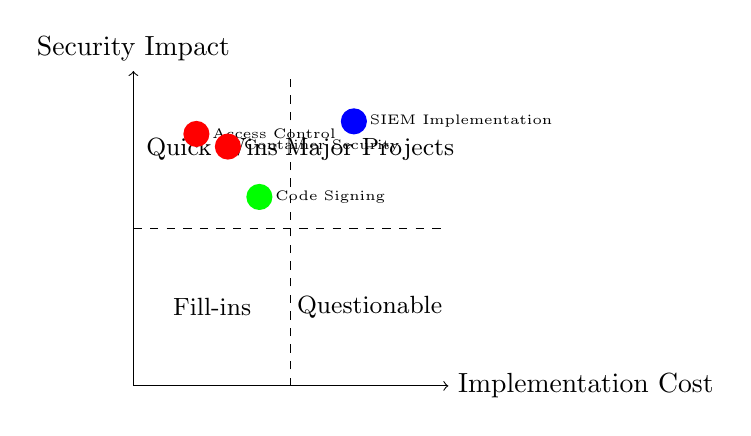
\begin{tikzpicture}[scale=0.8]
    % Risk/Impact Matrix
    \draw[->] (0,0) -- (5,0) node[right] {Implementation Cost};
    \draw[->] (0,0) -- (0,5) node[above] {Security Impact};
    
    % Quadrants
    \draw[dashed] (2.5,0) -- (2.5,5);
    \draw[dashed] (0,2.5) -- (5,2.5);
    
    % Quadrant labels
    \node at (1.25,3.75) {\small Quick Wins};
    \node at (3.75,3.75) {\small Major Projects};
    \node at (1.25,1.25) {\small Fill-ins};
    \node at (3.75,1.25) {\small Questionable};
    
    % Security measures plotted
    \node[circle, fill=red, minimum size=8pt] at (1,4) {};
    \node[right] at (1.1,4) {\tiny Access Control};
    
    \node[circle, fill=red, minimum size=8pt] at (1.5,3.8) {};
    \node[right] at (1.6,3.8) {\tiny Container Security};
    
    \node[circle, fill=blue, minimum size=8pt] at (3.5,4.2) {};
    \node[right] at (3.6,4.2) {\tiny SIEM Implementation};
    
    \node[circle, fill=green, minimum size=8pt] at (2,3) {};
    \node[right] at (2.1,3) {\tiny Code Signing};
\end{tikzpicture}
\caption{Sicherheitsmaßnahmen nach Kosten-Nutzen-Verhältnis}
\end{figure}

\subsection{Messbare Sicherheitsziele}

\begin{itemize}[leftmargin=*]
    \item \textbf{Reduzierung der Mean Time to Detection (MTTD)} von 24h auf <1h
    \item \textbf{Verbesserung der Mean Time to Containment (MTTC)} auf <15 Minuten
    \item \textbf{Erhöhung der Security Test Coverage} auf >90\%
    \item \textbf{Reduzierung kritischer Schwachstellen} um 95\%
    \item \textbf{Implementierung von 100\% Code-Signing} für Production-Builds
\end{itemize}

Das DVD-System demonstriert eindrucksvoll, wie scheinbar kleine Konfigurationsfehler zu katastrophalen Sicherheitslücken führen können. Die hier beschriebenen Defensive-Maßnahmen sind essentiell für den Schutz kritischer Drohnen-Infrastrukturen in Produktionsumgebungen.

\section{Anhang}

\subsection{Referenzen}

\begin{itemize}[leftmargin=*]
    \item MITRE ATT\&CK for ICS: \url{https://attack.mitre.org/matrices/ics/}
    \item NIST Cybersecurity Framework: \url{https://www.nist.gov/cyberframework}
    \item OWASP Container Security: \url{https://owasp.org/www-project-container-top-10/}
    \item CIS Docker Benchmark: \url{https://www.cisecurity.org/benchmark/docker}
    \item RTCA DO-326A/ED-202A: Airworthiness Security Process Specification
\end{itemize}

\subsection{Weitere Ressourcen}

\begin{itemize}[leftmargin=*]
    \item Drone Security Framework: \url{https://www.dronecode.org/security/}
    \item Industrial IoT Security: \url{https://www.isa.org/standards-and-publications/isa-standards/}
    \item Aviation Cybersecurity: \url{https://www.icao.int/cybersecurity/}
\end{itemize}

\end{document}